%!TEX root = ../report.tex


%%%%%%%%%%%%%%%%%%%%%%%%%%%%%%%%%%%%%%%%%%%%%%
\chapter{Delanalyse 2: Forskellen på et delmarked og et segment er påvisningen af særegne (specifikke? partikulære) sociale processer indenfor delmarkedet \label{kapitel_delanalyse2_socialeprocesser}}
%%%%%%%%%%%%%%%%%%%%%%%%%%%%%%%%%%%%%%%%%%%%%%

Efter at have konstateret at der er en opdeling af arbejdsmarkedet for arbejdstagere i delmarkeder, hvor mobilitet indenfor delmarkederne er hyppig, og mellem delmarkederne sjælden, har dette kapitel til formål at svare på det andet forskningsspørgsmål:

\begin{tcolorbox}[title=Forskningspørgsmål,
subtitle style={boxrule=0.4pt} ]
  \tcbsubtitle{2.} Kan forskelle i de sociale processer vise, at der er tale om segmenter, og ikke blot delmarkeder?
\end{tcolorbox}

Dette forskningsspørgsmål vil jeg besvare ved at kigge på de sociale processer i delmarkederne.

Lorem ipsum dolor sit amet, consectetur adipisicing elit, sed do eiusmod
tempor incididunt ut labore et dolore magna aliqua. Ut enim ad minim veniam,
quis nostrud exercitation ullamco laboris nisi ut aliquip ex ea commodo
consequat. Duis aute irure dolor in reprehenderit in voluptate velit esse
cillum dolore eu fugiat nulla pariatur. Excepteur sint occaecat cupidatat non
proident, sunt in culpa qui officia deserunt mollit anim id est laborum.



%%%%%%%%%%%%%%%%%%%%%%%%%%%%%%%%%%%%%%%%%%%%%%
\section{Indkomstfordeling for alle \label{sec_delanalyse2_loen_alle}}
%%%%%%%%%%%%%%%%%%%%%%%%%%%%%%%%%%%%%%%%%%%%%%



\begin{figure}
\parbox[H]{8cm}{\null
  % \centering
  \captionof{figure}{timeløn farvelagt efter udvalgte percentiler}
  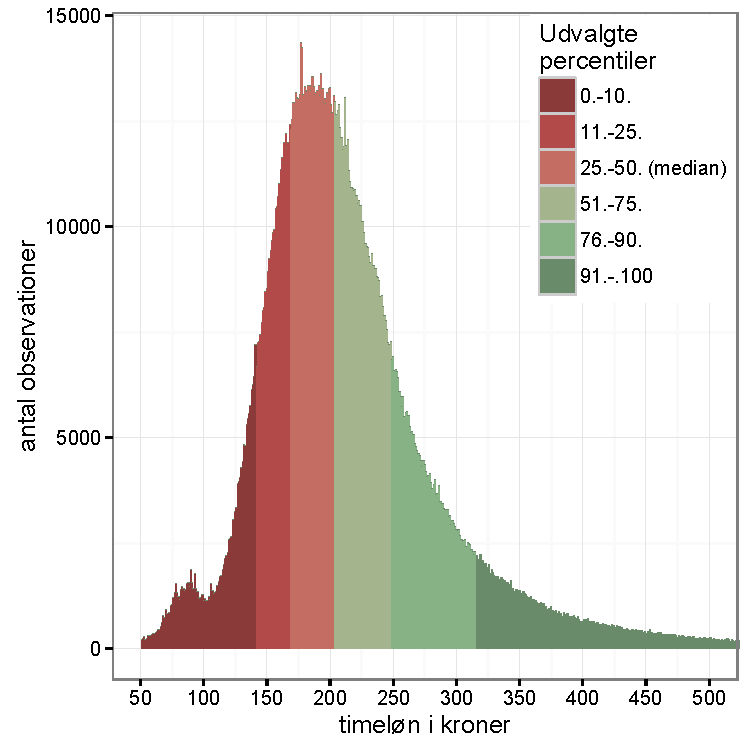
\includegraphics[width=7cm]{fig/deskriptive/timelon_quants_lowres2.pdf}
}
\parbox[H]{5cm}{\null
\centering
  % \vskip-\abovecaptionskip
  \captionof{table}[t]{Udvalgte mål for fordelingen af timelønninger \label{delanalyse2_timelon_fordelingogfigur}}%
  \vskip\abovecaptionskip
%
% Table generated by Excel2LaTeX from sheet 'delanalyse2_indkomstfordeling'
\begin{tabular}{lr}
\toprule
Gennemsnit &                    222 kr.  \\
Sd-afvigelse &                      76 kr.  \\
\midrule
Mindste værdi &                      18 kr.  \\
Højeste værdi &                 2.155 kr.  \\
\midrule
10. percentil &                    155 kr.  \\
25. percentil &                    177 kr.  \\
Median &                    207 kr.  \\
75. percentil &                    243 kr.  \\
90. percentil &                    302 kr.  \\
\midrule
\textit{n} & \textit{205.798} \\
\bottomrule
\end{tabular}%

%
}
\end{figure}
%


Indkomstfordelingen i den arbejdende del af den danske befolkning kan ses i figur \ref{delanalyse2_timelon_fordelingogfigur} og tabel \ref{delanalyse2_timelon_fordelingogfigur}. 

Vi kan se at fordelingen er nogenlunde centreret omkring gennemsnittet og medianen, hvilket også kommer til udtryk i standardafvigelsen på 76 kr/t. stigningen i timeløn fra 100 kr/t til 175 kr/t er drastisk, mens faldet fra omtrent 200 kr/t og fremefter er noget mere støt i hældningen. Det kan man tolke sådan, at arbejdsmarkedsinstitutioner og overenskomster er ganske effektive til at regulere løndannelsen, således at lave timelønninger alligevel hindres i at ramme de niveauer, som fri prissætningen på arbejdskraften ville medføre. Det ses også, af den lange hale i timelønfordelingens øvre percentiler, at en lignende mekanisme ikke findes for de højere indkomster. Det danske skattesystems progressive beskatning af indkomst har selvfølgelig en hvis betydning, men det har ikke på samme måde en tydelig opdæmmende effekt, som vi ser, at der må findes for de lavere timelønninger. det er tydeligt, at timelønninger over den 90. percentil, tjener eksponentielt mere og mere frem mod den højeste timeløn på 4.492 kr.

Derudover findes der en lille pukkel af løninger på mellem 25 og 75 kr%
%
\footnote{ Grundet en teknisk fejl, der ikke blev rettet inden min forbindelse til registerdata udløb, er lønninger mellem 25 og 50 kr/t ikke vist i grafen. Det betyder \emph{ikke} at de ikke er er tilstede i datamaterialet, blot at grafen ikke viser dem.}%
%
. Eftersom vores population er alle i arbejde melle 16 og 70 år, er der i de fleste tilfælde sandsynligvis tale om ungdoms- og studiearbejde. 

%
\section{indkomstfordelinger på delmarkederne \label{sec delanalyse2 loen paa delmarkederne} }
%

Efter at have set på fordelingen af timelønninger generelt, skal vi nu se hvordan det er er differentiereret ud fra arbejdsmarkedets delmarkeder og klynger.  

I figur \ref{fig_analyse_deskriptivt_kort_timelon} er netværkskortet farvelagt således, at hvid markerer medianen på 208 kr/t. De røde farver er timelønninger under 208 kr/t. Jo mørkere rød, desto lavere timeløn. De grønne farver er over 208 kr/t. Jo mørkere grøn, desto højere timeløn%
%
\footnote{ Delmarkeder med en gennemsnitlig timeløn på 350 kr/t er sat til 350, da skalen ville blive spredt for langt ud for at imødegå disse outliers, hvilket ville gøre det svært at se nuancerne i forskellen mellem de timelønninger, som de fleste erhvervsgrupper trods alt har.}%
%
. Det ses at den grønne farves graduering er strukket længere end rød. Det er ikke overraskende, da vi netop ud fra figur \ref{delanalyse2_timelon_fordelingogfigur} kan se, at timelønninger strækker sig lagnt højere op over medianen end under den, bl.a. grundet det danske arbejdsmarkedes indretning, som argumenteret for i beskrivelsen af figur \ref{delanalyse2_timelon_fordelingogfigur}.

%
\newgeometry{left=-0.01cm,bottom=0.1cm}
\begin{figure}[H]
\begin{center}
  \caption{Intern mobilitet for klyngerne.}
  \label{fig_analyse_deskriptivt_kort_timelon}
  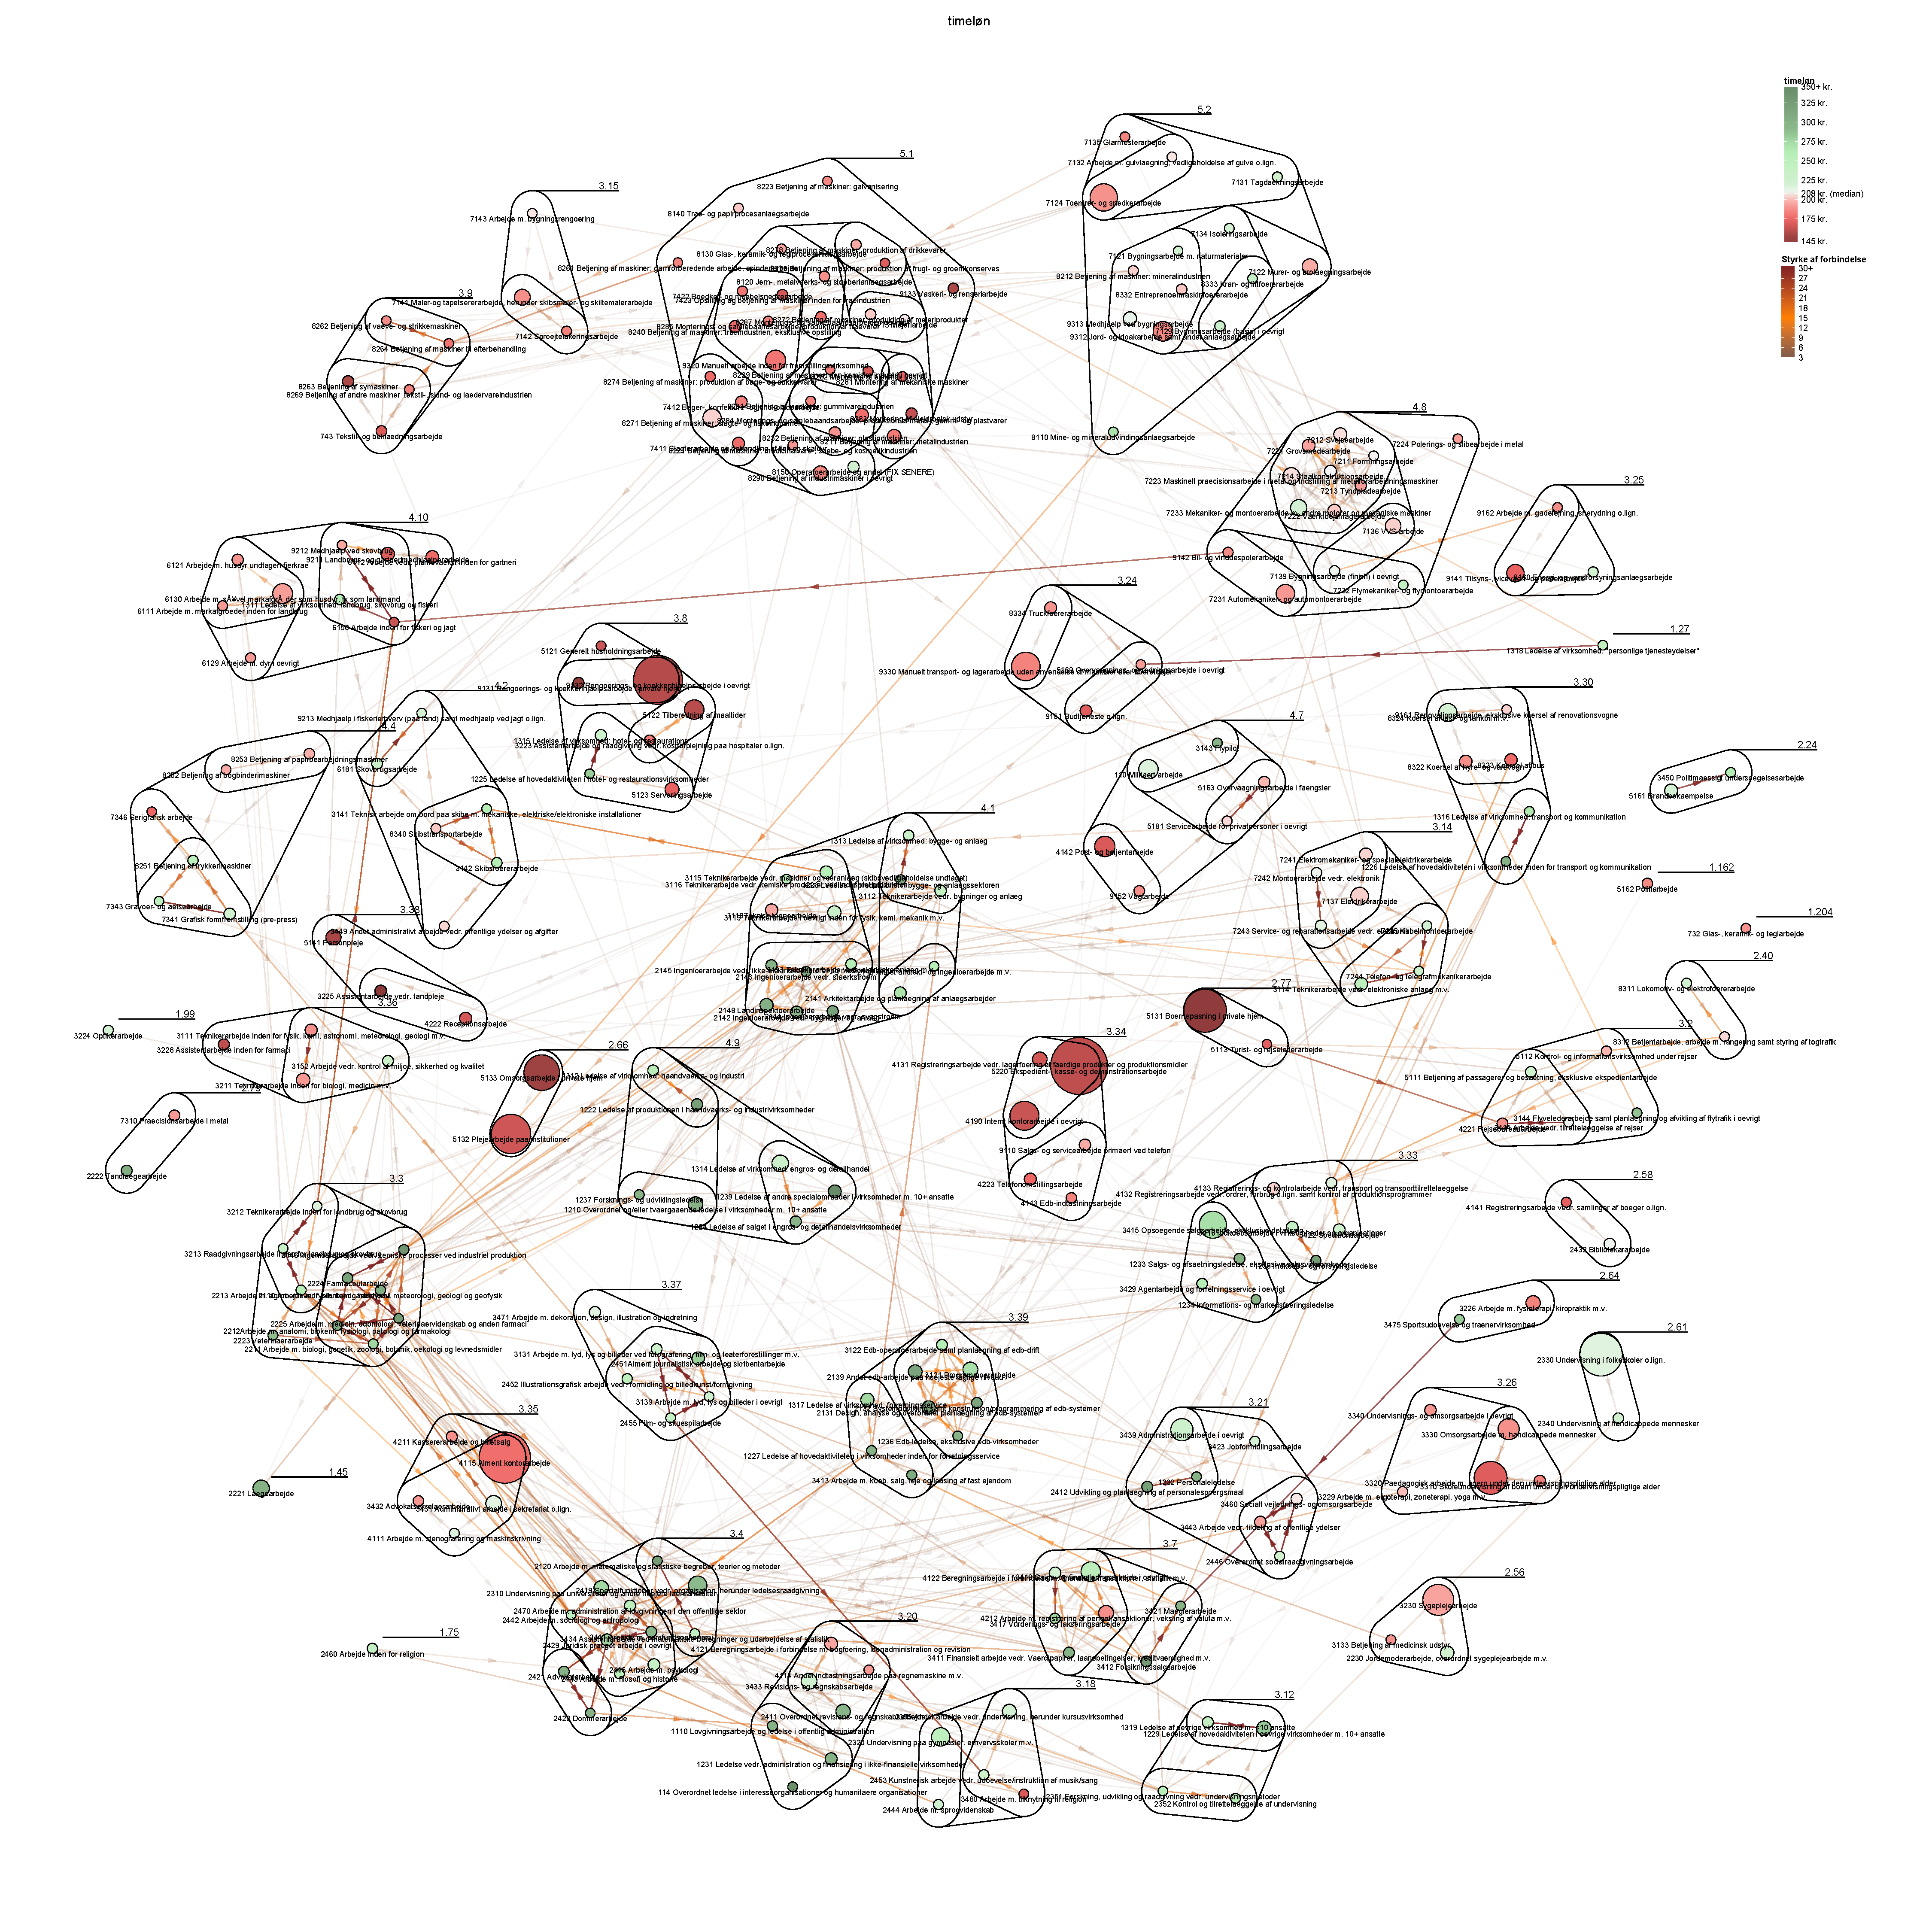
\includegraphics[width=1.0\textwidth]{fig/netvaerkskort/kort_timelon.pdf}
\end{center}
\end{figure}
\restoregeometry
%

Det overordnede netværkskort præsenteret her, giver os allerede en ide om en vis systematik i lønforholdene i forskellige placeringer på arbejdsmarkedet. Det er velkendt at kortets delmarkeder er lavet ud fra mobilitet mellem erhvervsgrupperne. Selve placeringen \emph{af} delmarkederne på kortet er imidlertidig også sket ud hvilken mobilitet der findes \emph{mellem} klyngerne. Derfor er det interessant, at vi ser en rødlig halvmåne forme sig i venstre side af kortet, mens en - lidt mindre - grøn formation findes i højre side. Ved at se på forbindelserne kan vi straks konstatere hvorfor, at kortet ser ud som det gør: Mellem de grønne, velbetalte delmarkeder ser vi meget kraftige forbindelser mellem delmarkederne. 

De 18 delmarkeder, der her er tale om, befinder sig stort set alle i Disco-hovedgruppe 1, 2 eller 3. Hvilket vil sige erhverv med høje (boglige) uddannelseskrav, og/eller meget ledelsesansvar. 

Der kan være to årsager til hvad vi ser på kortet: 1) Enten er udvekslingen af arbejdskraft på tværs af delmarkeder langt mere hyppig, eller 2) udvekslingen er mere specifik: Forbindelserne på kortet viser de kraftigste forbindelser, ikke alle forbindelser, og derfor vil mobilitet, der er mere jævnt fordelt, forblive usynlig på (denne udgave af) kortet. Ved at se på den interne mobilitet for sig for henholdsvis de 18 delmarkeder i den grønne formation for sig, og den røde halvmånes 36 delmarkeder for sig er det muligt at svare på. Den grønne formation har en gennemsnitlig intern mobilitet på 80 \%, og den røde halvmånes er på 77 \%%
%
  \footnote{ Det samme gælder for medianen og standardafvigelsen: Den røde halvmåne har en noget højere standardafvigelse og lavere median, men kun et par procentpoints forskel.}%
%
. Der er altså ikke tale om en væsentlig forskel i intern mobilitet mellem de to formationer. De kraftigere forbindelser i den grønne formation skyldes derfor, at den mobilitet, der findes, foregår langt mere struktureret langs bestemte linjer på tværs af delmarkederne. Den røde halvmånes mobilitet er “smurt tyndere ud”, og derfor ses den ikke på kortet%
%
 \footnote{ I appendiks \ref{app_netvaerkskort}, figur \ref{appendiks kort edges} findes et kort der viser alle forbindelserne, hvor dette kan ses.}%
%
.Sikft mellem den grønne formation af delmarkeder, med lange boglige uddannelse og/eller meget ledelsesansvar i højere grad sker via bestemte kanaler end tilfældet er i de resterende delmarkeder. Det er interessant, da det der netop karakteriserer den grønne formation, er at deres lønniveauer befinder sig i den bedst betalte halvdel af befolkningen. 

Hvis man skal komme med en tentativ analyse af hvad denne forskel i mobilitetsstruktur \emph{kan} betyde for den politiske orientering, erindrer læseren muligvis Claus Hjort Frederiksens udmelding som beskæftigelsesminister i 00'erne (find præcis årstal senere \#todo), hvor han kom i vælten ved at udtale, at hvis man med en lang videregående uddannelse ikke kunne finde job, skulle man finde arbejde i netto eller blive postbud i stedet. Det udløste et ramaskrig. Blandt dem med lang videregående uddannelse. Mens det for ikke-boglige klasser sandsynligvis var en ganske tilfredsstillende udmelding, og det er nok ikke usandsynligt, at udtalelser som denne, der gjorde Venstre til et bredt funderet parti i 00'ernes Danmark. Mit kort giver en troværdig forklaring på hvorfor, Da det ses, at netop erhvervsgrupper med lange videregående uddannelser, er vant til at søge beskæftigelse indenfor andre delmarkeder i langt mere strukturede baner end resten af delmarkederne. Det er denne form for kulturkrig, sociologen Thomas Frank beskriver i sin bourdieu-inspirerede klasseanalyse i bogen “What's the Matter with Kansas? - how the conservatives won the heart of America” fra \citeyear{Frank2007}. i Norge udkom en lignende bog i \citeyear{Marsdal2007} med en identisk Bourdieau-analyse, skrevet af journalisten Magnus  Marsdahl. Analysen er kort sagt, at venstrefløjspartierne er blevet til de boglige klassers parti. Det lukrerer de borgerlige politikere på ved at markerer sig med forslag og udtalelser, der er på kant med de “dannede” sociale gruppers verdensbillede, hvilket de naturligvis reagerer på med deres lærde sprog. Disse udmeldinger viser venstrefløjens traditionelle arbejderklasse, at den verden, hvori de venstreorienterede værdier står stærkt, ikke er deres verden. 

Det er selvfølgelig et noget stort brød at slå op, og jeg påstår ikke at den her fundne struktur kan bære en sådan bevisbyrde alene. Jeg vælger alligevel at præsentere den her, da jeg dog mener, at det netop er sådanne oplevelser af arbejdet, der giver et blik på verden, der kan formes til forskellige politiske perspektiver. Det er min overbevisning, at politiske værdiorienteringer ikke har samme kobling til arbejdslivet som tidligere, hvilket er et velfunderet empirisk standpunkt indenfor sociologisk og politologisk forskning (henvisning til Scott \#todo). Det betyder imidlertidig ikke, at politisk værdiorientering er \emph{af}koblet fra arbejdslivet, men at en række komplekse ændringer af parti, klasse og forbrugskulturen gør disse sammenhænge anderledes end tidligere. Som valget af Trump i november 2016 viste, er klasse stadig en relevant faktor, hvis man forstår hvad det betyder i dag (link til artikel fra Trumps datahold og så noget mere substantielt der viser at analytikerne tog fejl). Den her fremførte tolkning er et eksempel på hvorledes en oplevelse af arbejdslivet kan understøtte moderne sociologisk fundererede analyse om politisk værdidannelse ud fra moderne klasseteori, såsom Thomas Franks og Magnus Marsdahls analyser.



 % find ud af hvor meget mobilitet der "mellem" de to delmarkeder. \#todo 

%
\subsection{To delmarkeder i hver sin ende af indtjeningsspektret}
%

Hvilke delmarkeder har en høj timeløn og hvilke delmarkeder har en lav timeløn? Med andre ord - hvis vi starter helt naivt - er der bestemte typer arbejde, der er lønnes højt og lavt? Hvis vi antager, som Goldthorpe og Oesch gør det, at forskelligt arbejde indeholder forskellige sociale processer, må det være muligt at se dette afspejlet i delmarkedernes arbejdsindhold, samt hvor ens eller forskellige lønningerne er indenfor delmarkederne. 

 For at illustrerer det vil jeg zoomer ind på to delmarkeder, hvoraf et befinder sig i lave ende af timelønningerne og den anden i den højeste ende.

%
\subsubsection{Delmarked 3.35}
%



 Det første jeg vil fremhæve er delmarked \emak{s3.35}. Dette delmarked indeholder lavere grads servicejobs, og er det lavest lønnede delmarked, der består af > 2 erhvervsgrupper. Den gennemsnitlige timeløn, som aflæst i tabel, er på 175 kr/t, med en standardafvigelse på kun 14 kr/t. Der er tale altså tale om et delmarked, hvor gennemsnitslønnen er lav, og den er stabilt lav for alle de erhvervsgrupper, det består af. 
 % skal jeg lave en tabel med discogrupperne eller kun for segmentet? find ud af det senere \#todo

% Erhvervsgruppen består af jobbene telefonsælger, interviewer, pølsemand, klunser samt skopudser
Arbejdet i delmarkedet består af servicerelatereret arbejde, administrativt arbejde og kundepleje(?), og har ikke høje uddannelseskrav. Overraskende nok er det \emak{d9110} der har den højeste lønning på 197 kr/t. Det er overraskende, fordi erhvervsgruppen slet ikke har nogle uddannelseskrav, og er derfor i DSTs opdeling “færdighedsløst” arbejde. Denne erhvervsgruppe har dog også en intern højstandardafvigelse på 78 kr/t, den højeste i delmarkedet. Det giver god mening, da man må formode at der er stor forskel på at sælge hårde hvidevarer og sælge tekniske produkter til et nichemarked, hvor der kræves en vis teknisk kompetence for at kunne udtale sig om dets specifikationer. 

%
\begin{wrapfigure}{l}{6cm}
  \vspace{-20pt}
  \begin{center}
    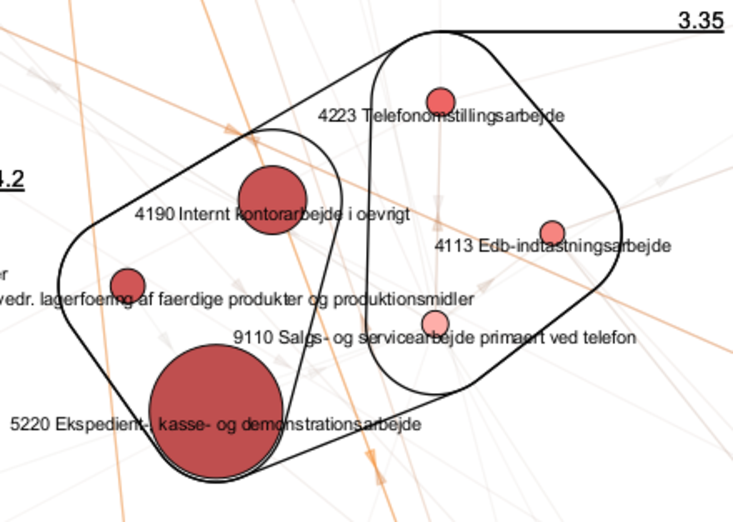
\includegraphics[width=6cm]{fig/segzoom/seg_3_35.pdf}
   \caption{}
   \label{fig_delanalyse1_zoom_3_35}
  \end{center}
  \vspace{-20pt}
\end{wrapfigure}
%

Delmarkedet er interessant af to simple årsager ud kvantitative mål, samt en enkelt teoretisk, der vokser ud af disse to. 

For det første indeholder den største enkeltstående erhvervsgruppe, \emak{5220},  der indeholder 5 \% af alle beskæftigede på det danske arbejdsmarked. Der er tale om en samling af jobs, der indeholder en lang en lang række ekspedientarbejde, såsom blomsterekspedient, købmandsekspedient, bilsælger og togsteward. Altså arbejde, hvor man sælger til, eller ekspedierer, kunder ansigt-til-ansigt. 

For det andet, grundet denne erhvervsgruppe er \emak{s3.35} det største delmarked, med 8 \% af det totale antal beskæftigede. Det er samtidig det delmarked, der har den ubetinget højeste andel af den totale mobilitet, på 8,8 \%, hvilket er 2,8 \% mere end det næststørste delmarked. 

For det tredje understøtte det Oesch tese om at skiftet fra produktion af fysiske varer til servicerelateret arbejde har betydning for klassestrukturen. Det er for tidligt at gå ind i endnu, men det er interessant, at det største \emph{og} lavest betalte delmarked er servicerelateret arbejde, hvis genstandsfelt er salg af varer til almindelige forbrugere. 

De nederste manuelle arbejdere i delmarked \emak{s5.1} der primært arbejder med betjening af maskiner i industriproduktionen, har faktisk en timeløn, der ligger 10 kr højere. Jeg vil uddybe dette senere, efter jeg har taget fat på hvad Oesch peger på som det andet vigtige parameter for den ændrede klassestruktur, som er kvindernes indtog på arbejdsmarkedet fra midten af det 20. århundrede og frem. 





%interessant nok er de også delt op i flere kategorier på 4-cifret niveau, hvor butiksassistent, blomsterekspedient, bilsælger etc er i samme kategori. Måske en blind vinkel i ISCED-klassifikationen. 
% dog ligger timelønnen for individer i segmentet på 264 i 3.35 og nærmest det samme i 5.1. jeg bruger gennemsnittet af erhvervsgrupper i stedet for individer fordi erhvervsgrupper er min analyseenhed, fuck individerne. det har den praktiske konsekvens at antallet af individer indenfor erhvervsgrupperne ikke medregnes i gennemsnittet for klyngerne, dvs hvis en af de erhvervsgruppe, dvs en af de 8 erhvervsgrupper, der indeholder < 600 personer var placeret i samme segment som en af de 8 erhvervsgrupper, der indeholder < 50.000, så ville gns for f.eks. løn være det samme.




%
\subsubsection{Delmarked 4.9}
%

Med 333 kr/t er delmarked \emak{s4.9} det bedst indtjenende delmarked i byen. Det indeholder $\nicefrac{1}{4}$ af erhvervsgrupperne i Discos hovedgruppe 1, som består af ledelse på øverste plan. Det har samtidig den 2. højeste standardafvigelse på 85 kr/t, så indtjeningen erhvervsgrupperne i mellem er meget varieret.  

% skriv noget her om ledelsesarbejde. Læs om ledelsesarbejde!           

Det er ikke overraskende at “ledelsesdelmarkedet” indtager denne position i indtjening. Det interessante er snarere, at de  resterende $\nicefrac{3}{4}$ indenfor ledelse på højeste plan er tilknyttet de delmarkeder, der relaterer sig til ledelsens genstandsfelt. Med andre ord er \emak{d1236} tilknyttet delmarked \emak{s2.31}, der har at gøre med det IT-udviklingsarbejde, der befinder sig på det “højeste” faglige niveau. Interessant nok gælder det også Disco 1-erhvervsgrupper, hvor det er ledelse af produktion, hvis arbejdskraft kræver mindre eksklusive kompetencer end i delmarkedet beskæftiget med IT-udvikling på højeste niveau. Eksempelvis landbrug, restauration og  %det skal nok ikke stå her, faktisk. 

%Måske skal jeg skrive om et andet delmarked i stedet, et der giver bedre mening. Hmmm. 

%                               ¤                             #


%
\begin{wrapfigure}{r}{6cm}
  \vspace{-20pt}
  \begin{center}
    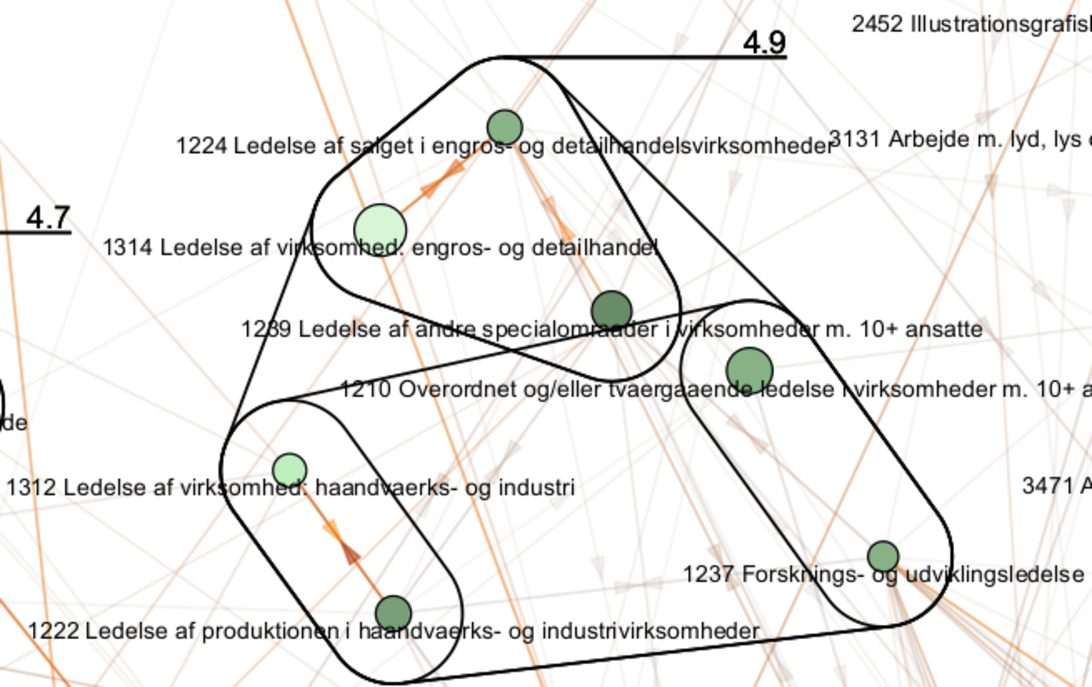
\includegraphics[width=6cm]{fig/segzoom/seg_4_9.pdf}
   \caption{}
   \label{fig_delanalyse1_zoom_4_9}
  \end{center}
  \vspace{-20pt}
\end{wrapfigure}
%




%%%%%%%%%%%%%%%%%%%%%%%%%%%%%%%%%%%%%%%%%%%%%%
\section{Kønsfordeling på arbejdsmarkedet \label{sec_}}
%%%%%%%%%%%%%%%%%%%%%%%%%%%%%%%%%%%%%%%%%%%%%%

først graf der viser stigning gennem min periode. citat om at kvindelig employment har været den største faktor employment i 80'erne og de tidlige 90'ere i vesteuropa, citat s. 33 Oesch.

udbudssiden er højere uddannelsesniveauer for kvinder, og steps toward equal right. på efterspørgselssiden er det væksten i servicejobsne der står for det. integrationen af husholdningsaktiviter i markedet og statsforbrug i offentlig sundhed og uddannelse har ændret efterspørgslen efter arbejdskraft og særligt kvindelig arbejdskraft markant. s. 33-4 

På demand siden


for klasseteori styrker casen for at den rette observationshed for klasse er individet, og ikke husholdningen. Mænds distribution på arbejdsmarkedet er anderledes end kvinders, og skal derfor forstås ud fra forskellige oplevelser af arbejdslivet. Når så mange kvinder arbejder i servicefag, er en opdeling baseret på manufaktur ikke til meget nytte når de skal placeres i et klasseskema. s. 35

Dette betyder også et skift fra hierarkisk stratifikation til horisontal stratifikation. 

fokus på husstand som observationsenhed eller individet stor splittelse i 80'erne. Mener med en vis form for konsensus om hvad formålet er, om det er at se på markedssituationen eller på arbejdssituationen. Individet er at foretrække på arbejdssistuationen, og det er den, jeg også vil fokusere på her. s. 42. 

"there are no grounds for regarding the lower leve ls o f  then on-manuel  hierarchyas somehow superior to manuel work" s. 46

Introduktionen af nye teknologier og automatiseringer gør at skellet mellem white-collar og blue-collar ændrer sig, den sociale distance mellem de to bliver anderledes. 




\iffalse
\label{iffalse}





De personer som arbejder og skifte job inden for delmarked \emak{s3.4} arbejder som advokater, dommere, sociologer, antropologer, statistikere, undervisere på universitetere, historikere, filosoffer, psykologer. De får en løn som i gennemsnit spænder fra XXX kr/time for de laveste (hvem er det) til XXX kr/time (hver er det). Udover en høj timeløn har de det til fælles at det typisk kræver en lang videregående uddannelser for at besidde disse job. Nogle jobs såsom advokat- og dommerarbejde har kræver udover en lang videregående uddannelser og en særlig efteruddannelse.

De personer som arbejder og skifte job inden for delmarked \emak{s5.1} arbejder som slagtere, bagere, mejerister, arbejde med betjening af maskiner, monteringsarbejde, samlebåndsarbejde og manuelt arbejde. De får en løn som i gennemsnit spænder fra XXX kr/time for de laveste (hvem er det) til XXX kr/time (hver er det) med en enkelt afstikker på XXX kr/time. Udover en lavere timeløn har de det til fælles at det typisk kræver en erhvervsuddannelse eller et kortere kursus at besidde disse job.

Den første umiddelbare umiddelbare forklaring på lønsforskellen mellem de to segmenter er uddannelse. For at arbejde inden for de to delmarkeder kræver det en uddannelse. Forskellen er så længden på uddannelsen. Det er anerkendt, at der er en sammenhæng mellem uddannelse er løn. Human kapital er en økonomisk teori udviklet af Gary Becker, der beskriver, at arbejdstagere kan tage en uddannelse som en investering mod forventning om økonomisk kompensation ved at vedkommendes produktivitet øges (fx Cahub og Zylberberg 2004, s. 69). Da de akademiske uddannelser tager længere tid end erhvervsuddannelser og kortere kursus, giver det også en højere økonomisk kompensation. 


%%%%%%%%%%%%%%%%%%%%%%%%%%%%%%%%%%%%%%%%%%%%%%
\newpage \section{Kønsforskelle blandt delmarkederne \label{sec_delanalyse2_loen}}
%%%%%%%%%%%%%%%%%%%%%%%%%%%%%%%%%%%%%%%%%%%%%%



Attributterne er ikke anvendt som inklusionskriterier og kan derfor bruges til at
vurdere, hvorvidt der er overensstemmelse mellem privilegerede positioner i netvær-
ket og symbolske eller økonomiske privilegier, der er eksterne for netværket. Dette giver
os mulighed for at vurdere om vores specifikation af netværket stemmer overens med
magtsymboler, hvilket kan benyttes til at vurdere validitet ( 1983, s. 29).


validitet i et klasseskema: ekstern og intern validitet (Oesch s. 94)

indkomst som udtryk for magt på arbejdsmarkedet og social status. Dermed "den afgørende faktor" for menneskers livschancer. s. 95

Boje peger på faren ved at fokusere på outcomet af sociale processer såsom lønforskelle, arbejdsløshed, hyppige jobskifte m.m.. Det er en reel fare ved mit empiriske arbejde. s. 28, men meget god hvis man vil sikre sig at alt er, som det skal være. 

Grundet den danske struktur og fokus på organisering må det forventes, at mobilitets- og lønbarrierer primært findes indenfor fag, og ikke indenfor industrier/erhvervsgrene, hvilket findes i USAs langt mindre organiserede og mere monopolitiske virksomhedskultur. 

"i perioder med økonomisk tilbagegang og hvor der på arbejsmarkedet er overudbud af lønarbejdere synes barriererne mellem segmenterne at blive skærpet." (...) og nye segmenter og delmarkeder opstår på den baggrund. s. 72
→ perioden 1996-2009 er en periode med vækst, dvs: Det her en god periode. Find tal for økonomisk vækst for perioden


brug relative forskel mellem lønninger, ikke bare den absolutte, som må siges at være den vigtigste for personerne selv. Brug medianen for den "nederste klasse" som udtryk for lønniveauet. Kan du overføre det til dit eget? lønniveauet for den lavest tjenende klynge?

Oesch afviser at "future prospects" skulle have stor betydning, da han mener at påvise en stærk sammenhæng mellem nuværende lønninger og fremtid indkomst. I danmark, viser Esping-Andersen, fungerer low-income jobs sådan. Men vi kan jo se, hvor folk bevæger sig hen. Og det ser ikke ud til at være en stærk sammenhæng mellem service-jobs og future prospects. Undersøg servicejobs og ande


find ud af hvor mange skift der er per år. Dejligt konkret tal. henvis til boje 1988 s. 123


Løndannelsen s. 79-80
	i det sekundære arbejdsmarked synes der ikke at være en sammenhæng mellem løn og uddannelse - det er ikke det, der er det centrale. Hvorimod på det primære arbejdsmarked synes det netop at være betydningsfuldt, her er uddannelsesmæssige ressource nøje afstemt med løn. 
	tre forhold spiller ind:
	- institutionel regulering kontra markedsregulering: I DK er stort set al løndannelse reguleret gennem institutionelle aftaler 
	→ har nok ændret sig noget siden, men i det store og hele nok stadig rigtigt
	- Lønnen knyttet til job kontra til præstation.
	- lønnen tilnyttet stillingsmæssigt avancement/ikkeavancement. primære forskel på sekundær/primær løn. det sekundære jobmarked har samme lønninger livet igennem. 





















% %%%%%%%%%%%%%%%%%%%%%%%%%%%%%%%%%%%%%%%%%%%%%%
% \section{kønsforskelle i sociale processer \label{sec_delanalyse2_køn}}
% %%%%%%%%%%%%%%%%%%%%%%%%%%%%%%%%%%%%%%%%%%%%%%

% En grundlæggende differentieringsform i snart sagt alle samfund er



%  kønsopdelingen, der kommer til udtryk i en kønsbestemt arbejdsdeling i langt de fleste samfund. Som David Oesch bemærker, er det påfaldende, hvor få kvantitative undersøgelser af arbejdsmarkedsrelationer, der inddrager køn i analyserne  














\fi


